\documentclass[aspectratio=169,xcolor=dvipsnames]{beamer}

\usepackage{hyperref}
\usepackage{graphicx}
\usepackage{booktabs}



\title[short title]{Bridging the Gap: Analyzing Auction Prices and Day-Ahead Market Discrepancies at the Swiss-German Electricity Border}

\author{Nicolas Greber, Massimo Nardo, Vansh Khanna}
\institute
{
    Department of Finance \\
    University of Zurich
    \vskip 3pt
}
\date{\today}



\begin{document}

\begin{frame}
    \titlepage
\end{frame}

\begin{frame}{Overview}
    \tableofcontents


\end{frame}

\section{Background and Motivation}
\begin{frame}{Background and Motivation}
\begin{itemize}
    \item \textbf{Day-ahead electricity markets} allow electricity to be traded for delivery the following day (single hours).
    \item \textbf{Germany-Luxembourg} is a market with its own price for electricity delivered there, and \textbf{Switzerland} is a separate market with its own price for electricity delivered there.
    \item \textbf{Limited cross-border capacity} is auctioned by the Joint Allocation Office (JAO) for electricity to be imported/exported the following day (single hours).
    \item An \textbf{arbitrage argument} suggests that border prices should align with day-ahead market price differences.
    \item \textbf{Mispricing} at the border could reveal \textbf{market inefficiencies} and provide insights for improving integration.
\end{itemize}
\end{frame}


\section{Hypotheses}
\begin{frame}{Hypotheses}
\begin{itemize}
    \item \textbf{The Convergence Hypothesis:}  
    The price difference between Germany and Switzerland, adjusted for border costs in both directions, equals zero. This equilibrium arises from arbitrage opportunities and the absence of transaction costs in JAO auctions.
    
    \item \textbf{The Independence Hypothesis:}  
    Any observed pricing errors are uncorrelated over time, indicating no systematic patterns in their occurrence.
    
    \item \textbf{The Volatility Growth Hypothesis:}  
    Pricing accuracy has deteriorated as solar capacity expansion creates more unpredictable supply-demand patterns.
\end{itemize}
\end{frame}

\section{Data}
\begin{frame}{Data}
\begin{itemize}
    \item \textbf{Day-Ahead Market Prices (hourly):}
    \begin{itemize}
        \item Covers Switzerland, Germany-Luxembourg, and Germany-Austria-Luxembourg.
        \item Dataset: 2016–2023 (restricted to 2019–2023 for consistency).
        \item Settlement times:
        \begin{itemize}
            \item Switzerland: 11:00 CET.
            \item Most European markets: 12:00 CET.
        \end{itemize}
    \end{itemize}
    \item \textbf{Cross-Border Auction Prices (hourly):}
    \begin{itemize}
        \item From Joint Allocation Office (JAO).
        \item Allocate daily transmission capacity; auctions close at 09:30 CET.
        \item Each unit represents 1 MWh of electricity.
        \item Data: 2019–2023 (via JAO API).
    \end{itemize}
    \item \textbf{Photovoltaic (PV) Data (yearly):}
    \begin{itemize}
        \item From Swiss Federal Office of Energy (SFOE).
        \item Includes installed PV capacity and number of installations.
        \item Supports analysis of renewable energy impact on pricing.
    \end{itemize}
\end{itemize}
\end{frame}

\section{Methodology}
\begin{frame}{Methodology}
\begin{itemize}
    \item \textbf{Key Variables:}
    \begin{itemize}
        \item Hourly Day-ahead prices (\( p_t^{CH}, p_t^{DE} \)) 
        \item Hourly Cross-border auction prices (\( p_t^{CH \rightarrow DE}, p_t^{DE \rightarrow CH} \)).
    \end{itemize}
    \item \textbf{Error Terms:}
    \begin{itemize}
        \item Pricing deviation: 
        \[
        \delta_t = p_t^{DE} + p_t^{DE \rightarrow CH} - p_t^{CH} - p_t^{CH \rightarrow DE}.
        \]
        \item Normalized deviation: 
        \[
        \hat{\delta}_t = \frac{\delta_t}{(p_t^{CH} + p_t^{DE})/2}.
        \]
    \end{itemize}
    \item \textbf{Statistical Tests:}
    \begin{itemize}
        \item \textit{Stationarity:} Does $\delta_t$ revert to a mean (temporary inefficiencies) or persist (structural issues)?
        \item \textit{Mean test:} Is $\mathbb{E}[\delta_t] = 0$, indicating no systematic mispricing?
        \item \textit{Autocorrelation:} Are pricing deviations correlated over time (e.g., at daily lags)?
        \item \textit{Variance trend:} Does the variability of normalized deviations ($\hat{\delta}_t$) increase over time?
    \end{itemize}
\end{itemize}
\end{frame}

\section{Results}

\begin{frame}{Results I: Observable Dynamics}
    \begin{center}
        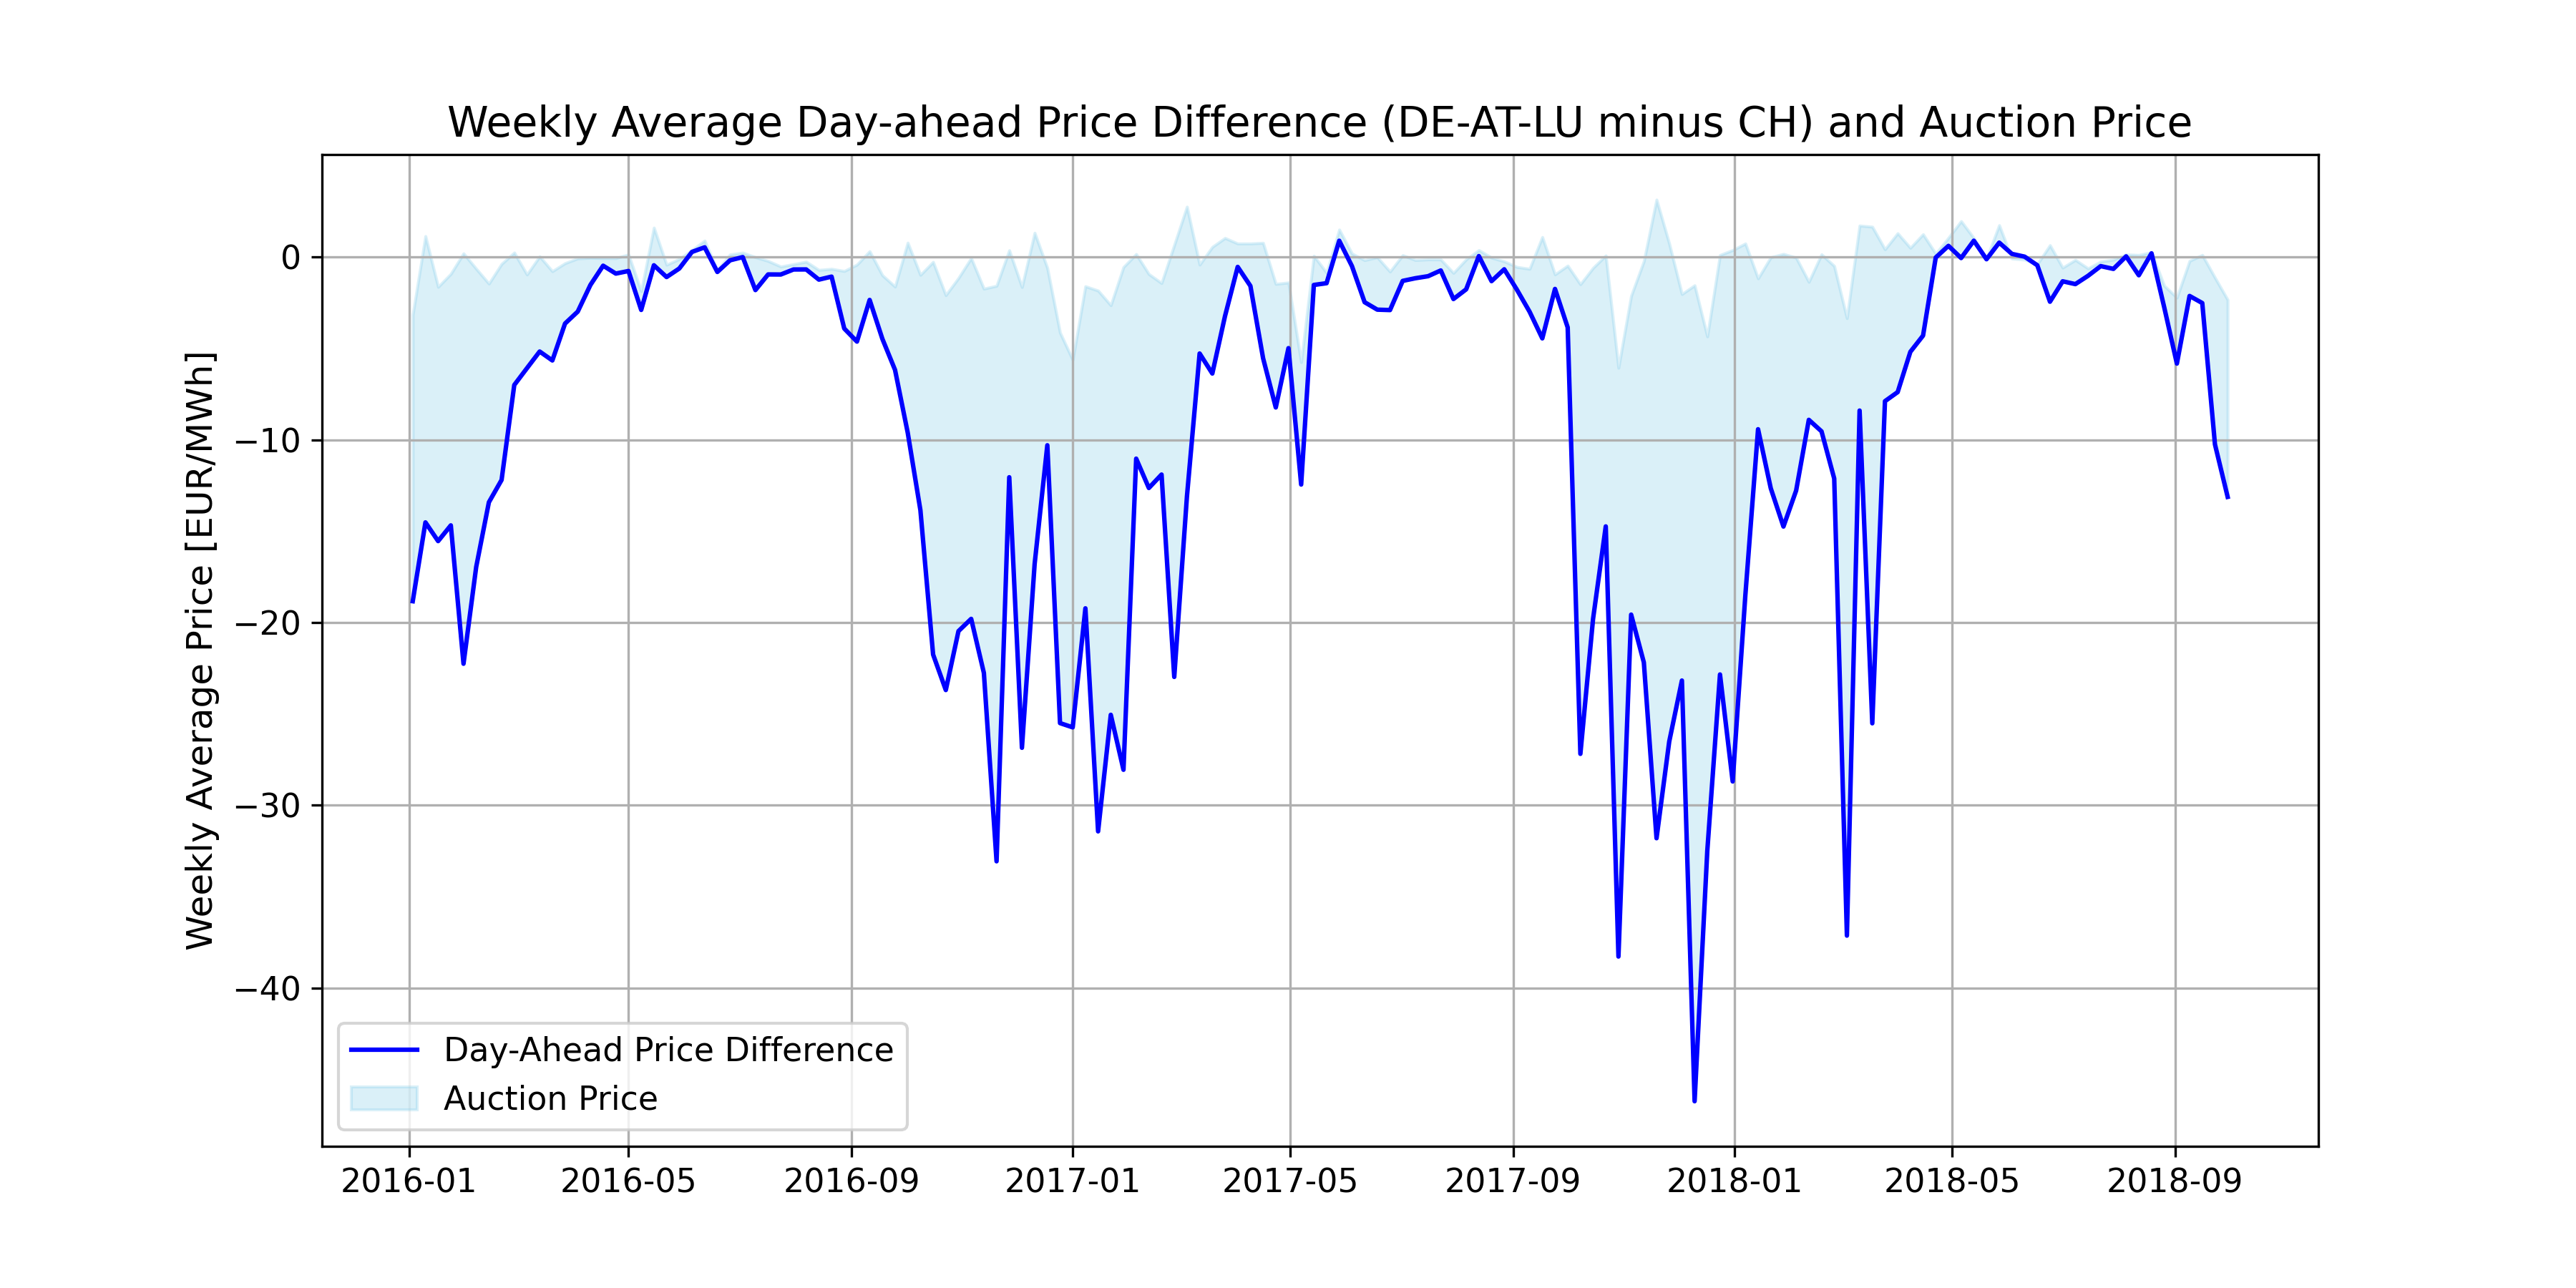
\includegraphics[width=\textwidth]{figures/weekly_average_day_ahead_price_diff_de-lu-at_ch.png}
    \end{center}
\end{frame}

\begin{frame}{Results II: Observable Dynamics}
    \begin{center}
        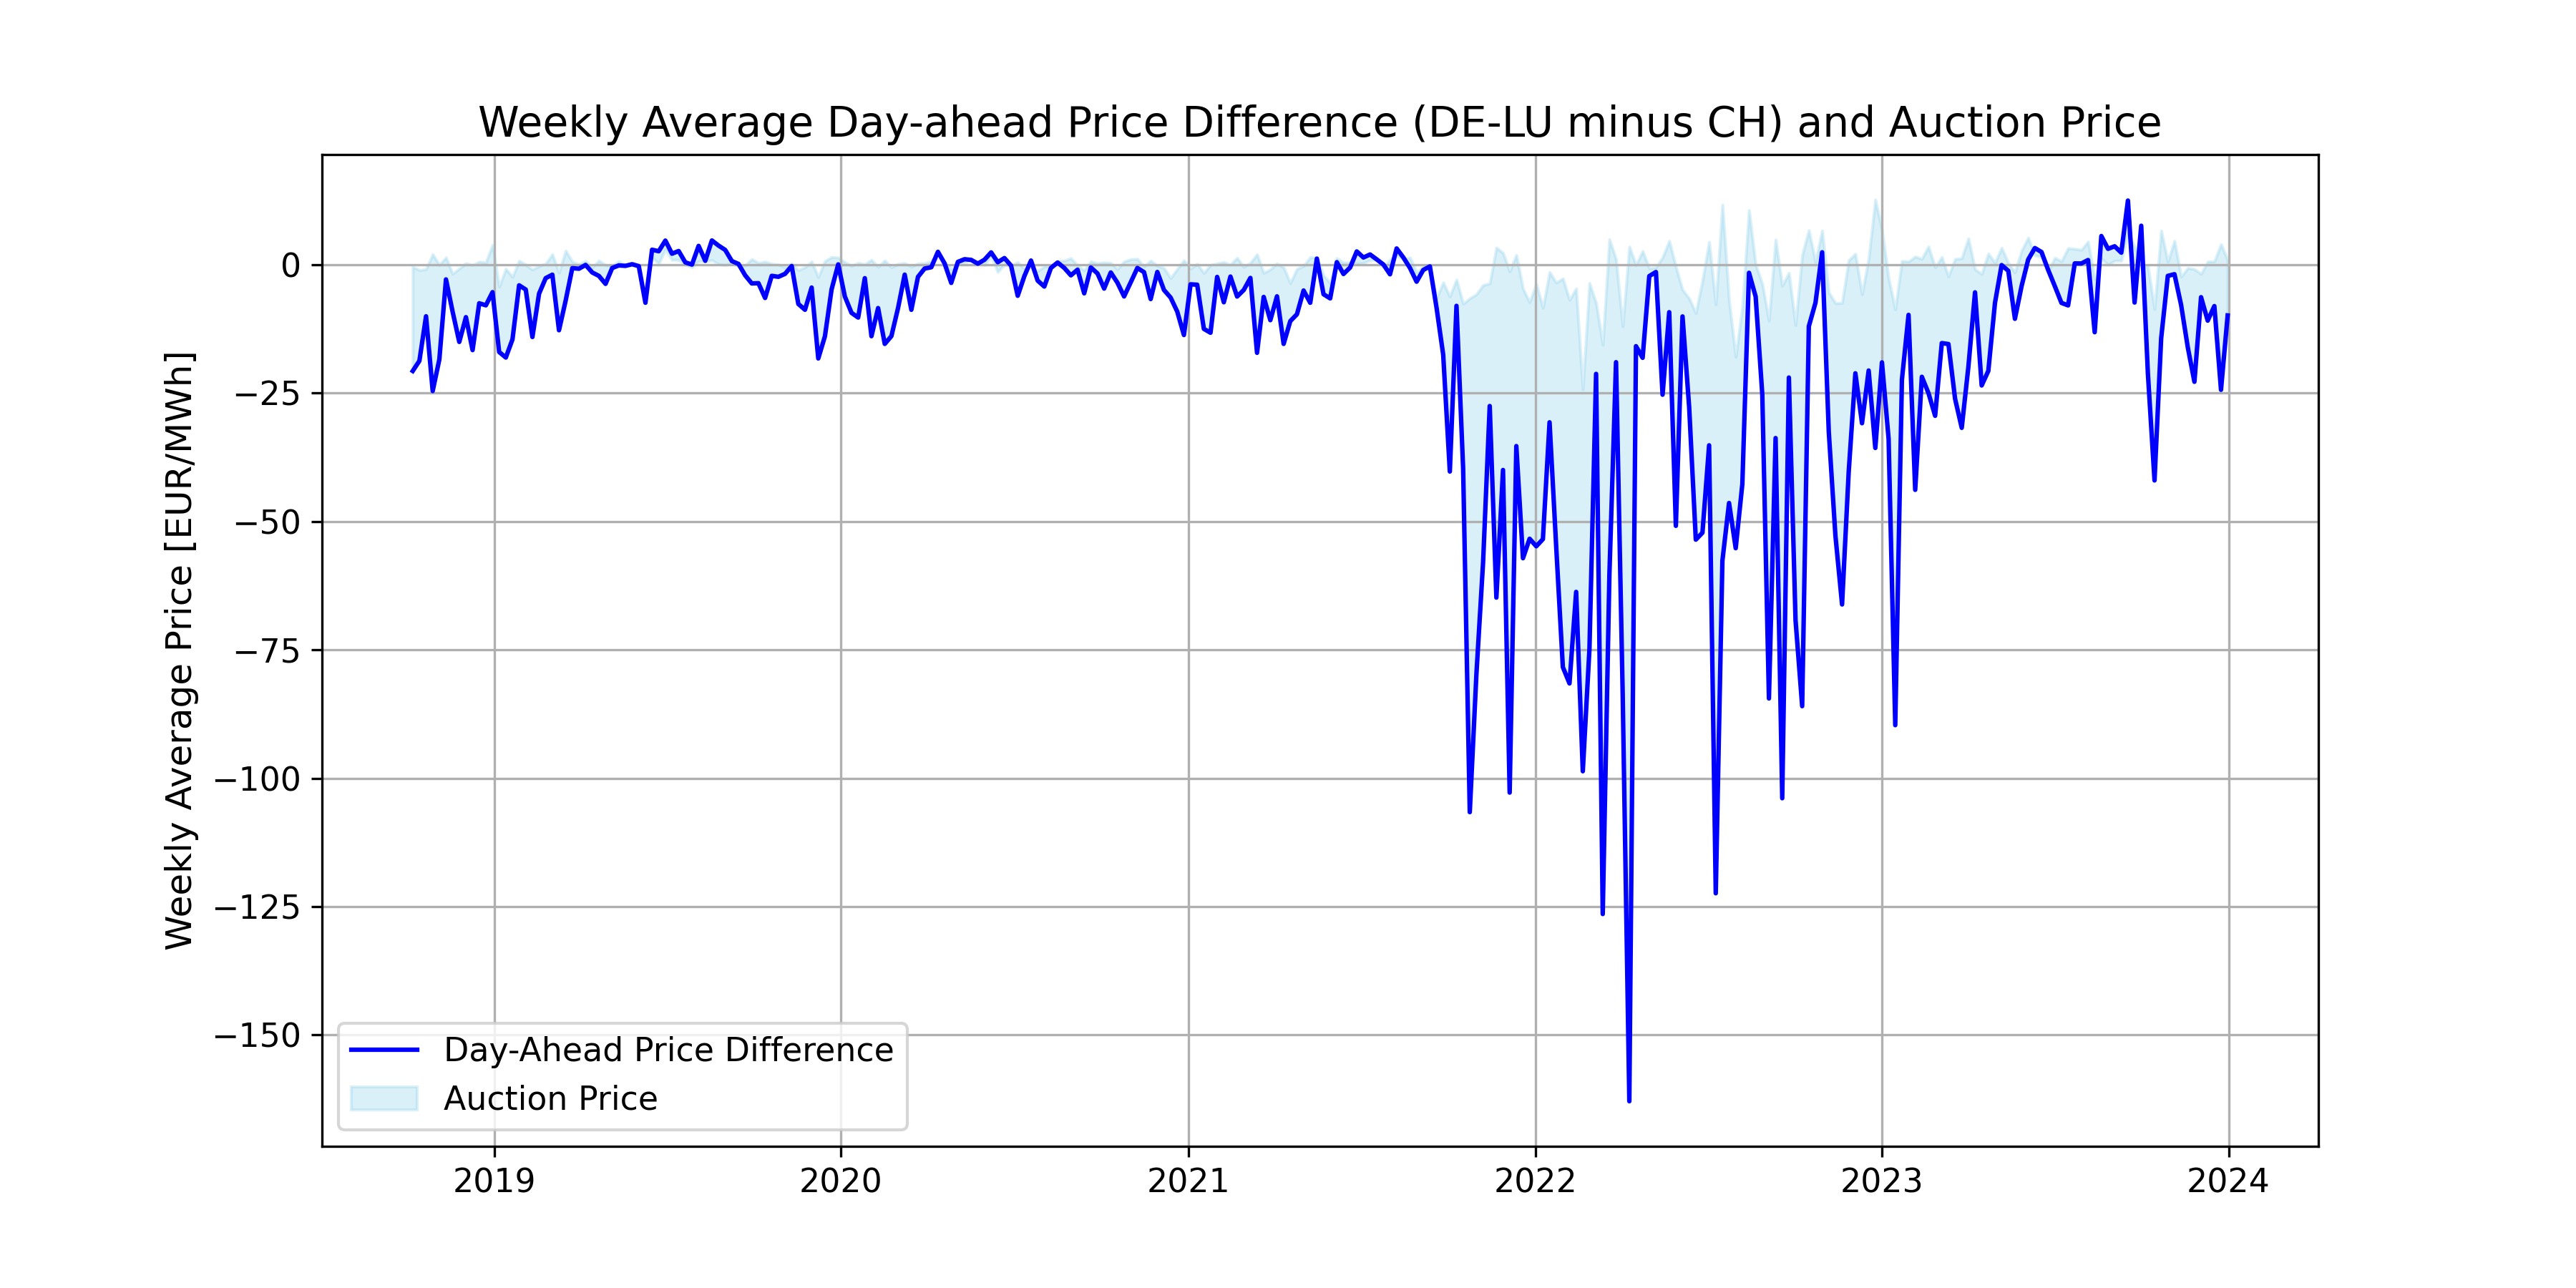
\includegraphics[width=\textwidth]{figures/weekly_average_day_ahead_price_diff_de-lu_ch.png}
    \end{center}
\end{frame}


\begin{frame}{Results III: Analysis}
\begin{columns}
    \begin{column}{0.4\textwidth}
    \footnotesize
        \textbf{Key Insights:}
        \begin{itemize}
            \item \textbf{Convergence:} ADF test confirms stationarity ($p < 0.001$), supporting mean-reverting price deviations.
            \item \textbf{Inefficiencies:} HAC test shows small but significant mean deviation ($p < 0.05$), suggesting systematic biases.
            \item \textbf{Temporal Patterns:} Significant autocorrelation at lag 24 ($p < 0.001$), indicating daily cycles in errors.
            \item \textbf{Volatility Growth:} No trend in variance over time ($p = 0.959$); variance ratio test shows an increase ($p < 0.001$), linked to PV expansion or market stress.
        \end{itemize}
    \end{column}

    \begin{column}{0.6\textwidth}
        \centering
        \scriptsize
        \begin{table}[ht]
           \caption{Statistical Test Results}
           \label{tab:test_results}
           \begin{tabular}{lrrc}
               \hline
               \textit{Test} & \textit{Value} & \textit{P-value} & \textit{Inference} \\
               \hline
               ADF Test & -26.112 & 0.000 & Stationary \\
               HAC Test & 2.175 & 0.030 & Mean deviation \\
               Autocorr. (Lag 24) & 0.021 & 0.000 & Serial correlation \\
               Variance Trend & 1.00e-5 & 0.959 & No trend \\
               Variance Ratio & 2.685 & 0.000 & Variance increase \\
               \hline
           \end{tabular}
        \end{table}
    \end{column}
\end{columns}
\end{frame}

\begin{frame}{Results IV: Yearly Analysis}
\begin{columns}
    \begin{column}{0.5\textwidth}
    {\footnotesize
            \textbf{HAC Results:}
            \begin{itemize}
                \item 2019–2020: Mean deviations are insignificant ($p > 0.05$), indicating negligible pricing errors under normal conditions.
                \item 2021–2023: Significant deviations ($p < 0.05$), aligning with market volatility during the energy crisis, suggesting inefficiencies in stressed periods.
            \end{itemize}
            \textbf{Autocorrelation:}
            \begin{itemize}
                \item 2019–2020: Significant daily cycles ($p < 0.01$)
                \item 2021–2023: Decreasing significance ($p > 0.1$ in 2022–2023), indicating fewer systematic patterns.
            \end{itemize}}
    \end{column}

    \begin{column}{0.5\textwidth}
        \centering
        \scriptsize
        \begin{table}[ht]
           \caption{Yearly Statistical Test Results}
           \label{tab:yearly_test_results}
           \begin{tabular}{l|rr|rr|rr}
               \hline
               \textit{Year} & \textit{HAC t-stat} & \textit{p-val} & \textit{Autocorr} & \textit{p-val} \\
               \hline
               2019 & -0.295 & 0.768 & -0.048 & 0.000 \\
               2020 & -1.117 & 0.264 &  0.032 & 0.003 \\
               2021 &  2.903 & 0.004 &  0.026 & 0.015 \\
               2022 &  2.557 & 0.011 &  0.016 & 0.138 \\
               2023 & -2.341 & 0.019 &  0.017 & 0.121 \\
               \hline
           \end{tabular}
        \end{table}
    \end{column}
\end{columns}
\end{frame}

\begin{frame}{Results V: Evaluation of Hypotheses}
\textbf{Convergence Hypothesis:}
\begin{itemize}
    \item Stationarity of $\delta_t$ (ADF test) confirms temporary, mean-reverting price deviations, even during the 2022 energy crisis.
    \item Significant mean deviations (HAC test) in 2021–2022 suggest inefficiencies, possibly due to market stress or structural constraints.
\end{itemize}

\textbf{Independence Hypothesis:}
\begin{itemize}
    \item Significant autocorrelation (lag 24) in 2019–2020 indicates daily cycles and systematic dependencies in pricing errors.
    \item Reduced autocorrelation from 2021 onward reflects potential improvements in forecasting and market responses.
\end{itemize}

\textbf{Volatility Growth Hypothesis:}
\begin{itemize}
    \item No significant linear volatility growth (trend test) across the study period.
    \item Variance increase (ratio test) in 2022–2023. However, it is not clear whether the increase stems from an increase in PV or other factors. 
\end{itemize}
\end{frame}

\begin{frame}{Conclusion and Outlook}
\textbf{Key Takeaways:}
\begin{itemize}
    \item Cross-border electricity markets exhibit mean-reverting price deviations, supporting the convergence hypothesis.
    \item Temporal dependencies highlight early inefficiencies, but recent improvements suggest adaptive market responses.
\end{itemize}
\vspace{1cm}
\centering
\textit{Thank you for your attention!}
\end{frame}



\end{document}